\documentclass{llncs}

\usepackage[T1]{fontenc}
\usepackage{amsmath}
\usepackage{amssymb}
\usepackage{graphicx}
\usepackage{hyperref}
\usepackage{subcaption}

\begin{document}

% title header
\title{Continual Reinforcement Learning for Evolving Games: Learning Across Game Updates in Competitive Pokémon}
\author{Thomas Vroom, Dennis J.N.J. Soemers}
\institute{Department of Advanced Computing Sciences\\Maastricht University\\Maastricht, The Netherlands\\\email{\{thomas.vroom,dennis.soemers\}@maastrichtuniversity.nl}}
\maketitle

\paragraph{Introduction}
Many modern live-service games receive frequent updates that modify existing game mechanics, intentionally altering the strategic landscape to maintain competitive balance and player engagement~\cite{chitayat2023gameupdates}.
This poses a major challenge for the development of competitive Reinforcement Learning (RL) agents, whose learned strategies may suddenly be invalidated by these updates.
Alternatively, training agents from scratch after every update is computationally expensive, and might discard valuable knowledge acquired from previous versions of the game.
Continual Reinforcement Learning (CRL) aims to enable agents to acquire new knowledge while retaining previously learned capabilities, allowing them to adapt to a sequence of tasks or domains over time~\cite{wang2024cl}.
We investigate whether CRL can facilitate effective knowledge transfer across game updates.
The domain of this work is competitive Pokémon (VGC), a challenging environment that sees natural non-stationarity through seasonal rulesets, called \textit{``regulations"} (\textbf{A}-\textbf{J})~\cite{angliss2025vgc,vgc-rules-regulations}.

\paragraph{Methods}
Our work is built on top of \textit{VGC-Bench}, a comprehensive VGC benchmark that introduces transformer-based self-play RL agents capable of beating human VGC players~\cite{angliss2025vgc}.
Starting with RL agents trained exclusively on regulation \textbf{A}, we show that these agents can successfully transfer knowledge short-term to future regulations using full fine-tuning, but lose out to retrained agents after repeated transfer due to loss of plasticity and unstable value predictions.
To address the instability concerns, we propose two adjustments to VGC-Bench's policy architecture: changing the Gaussian initialization of the embeddings from $\mathcal{N}(0,1)$ to $\mathcal{N}(0,0.02)$, and changing the gain of the orthogonal initialization of the linear layer projecting the transformer output to value predictions from 1 to 0.01.
We also identify \textit{Progressive Neural Networks}~\cite{rusu2016pnn} and \textit{Tuned PPO} (adjusted Adam $\beta$s and L2 regularization, optimized for retaining plasticity)~\cite{dohare2024plasticity,lyle2023plasticity} as promising techniques for mitigating loss of plasticity in VGC.
We adapt these methods to VGC-Bench's policy architecture and compare them to full fine-tuning and complete retraining when transferring from regulation \textbf{A} to \textbf{B}, to \textbf{C}, etc.
The results are shown in Figure~\ref{fig:results}.

\newpage
\begin{figure}[ht]
    \centering
    \begin{subfigure}{.475\textwidth}
        \centering
        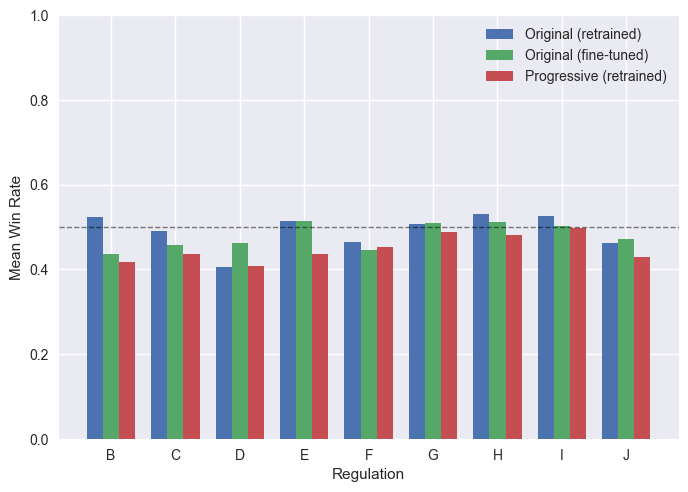
\includegraphics[width=\textwidth]{images/progressive-indist.png}
        \caption{Agents with a progressive architecture, evaluated using teams seen during training.}
        \label{fig:progressive-indist}
    \end{subfigure}
    \hfill
    \begin{subfigure}{.475\textwidth}
        \centering
        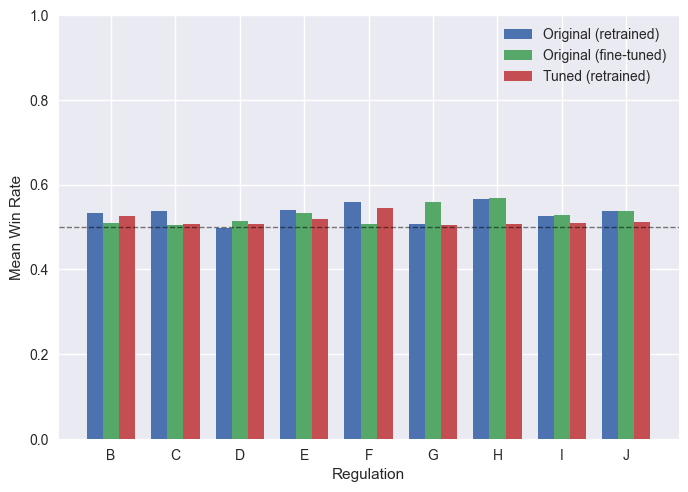
\includegraphics[width=\textwidth]{images/tuned-indist.png}
        \caption{Agents trained using tuned PPO, evaluated using teams seen during training.}
        \label{fig:tuned-indist}
    \end{subfigure}
    \vskip\baselineskip
    \begin{subfigure}{.475\textwidth}
        \centering
        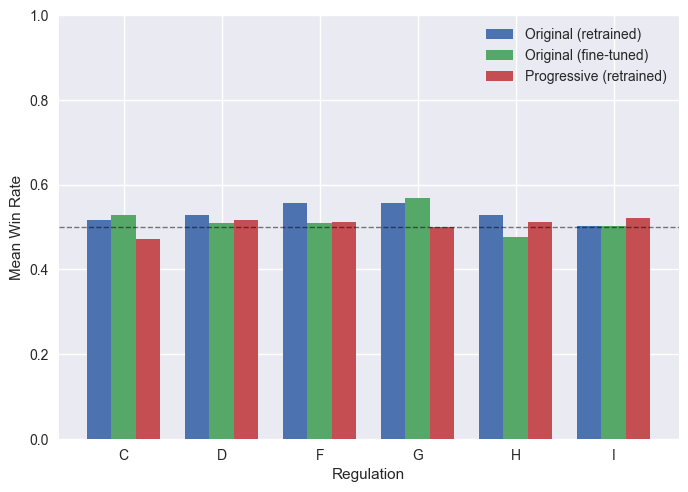
\includegraphics[width=\textwidth]{images/progressive-outofdist.png}
        \caption{Agents with a progressive architecture, evaluated using teams \textit{not} seen during training.}
        \label{fig:progressive-outofdist}
    \end{subfigure}
    \hfill
    \begin{subfigure}{.475\textwidth}
        \centering
        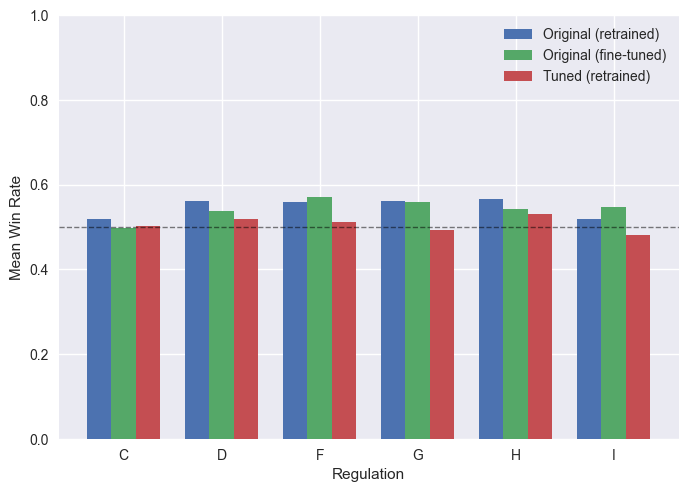
\includegraphics[width=\textwidth]{images/tuned-outofdist.png}
        \caption{Agents trained using tuned PPO, evaluated using teams \textit{not} seen during training.}
        \label{fig:tuned-outofdist}
    \end{subfigure}
    \caption{Mean win rates of our agents against VGC-Bench's original agents retrained (blue/left), VGC-Bench's original agents fine-tuned (green/middle), and our agents retrained (red/right). Evaluated over 1000 episodes.}
    \label{fig:results}
\end{figure}

\paragraph{Conclusion}
Figures~\ref{fig:tuned-indist} and~\ref{fig:tuned-outofdist} show that, compared to the original agents, our proposed policy adjustments together with tuned PPO facilitates a better knowledge transfer across regulations.
Figures~\ref{fig:progressive-indist} and~\ref{fig:progressive-outofdist} show that, while the progressive architecture does not suffer from loss of plasticity, it does not facilitate a better knowledge transfer when evaluating using the same teams as seen during training.
Overall, our agents are not able to consistently outperform retrained agents of the same architecture, indicating that complete retraining remains the most effective approach for mitigating non-stationarity in VGC.
Nevertheless, our proposed methods consistently improve the outright performance and generalization to unseen teams compared to VGC-Bench's original agents, suggesting that continual learning is still beneficial to RL agents in VGC.

% references
\newpage
\bibliographystyle{splncs04}
\bibliography{bibliography}

\end{document}
